\documentclass[11pt,aspectratio=169]{beamer}
\usetheme{default}
\usecolortheme{beaver}
\setbeamertemplate{navigation symbols}{}
\setbeamertemplate{footline}[frame number]
\usepackage{amsmath,amssymb,booktabs,tikz}
\usetikzlibrary{arrows.meta,positioning}
\graphicspath{{figs/}}

\newcommand{\Ham}{H}
\newcommand{\Zhat}{\widehat{\mathbb Z}}
\newcommand{\KL}{\mathrm{KL}}
\newcommand{\proved}{\textcolor{green!50!black}{\textbf{[proved]}}}
\newcommand{\computed}{\textcolor{blue!70!black}{\textbf{[computer-verified]}}}
\newcommand{\conj}{\textcolor{red!70!black}{\textbf{[conjecture]}}}
\newcommand{\heur}{\textcolor{orange!80!black}{\textbf{[heuristic]}}}

\title{Counting square chains}
\subtitle{lifts, limits, and an entropy conjecture}
\author{Victor S. Miller}
\date{}

\begin{document}

\begin{frame}
\titlepage
\end{frame}

%=====================================================================
\begin{frame}{Square chains}
$G(n)$: vertices $1,\dots,n$; \quad $i\sim j \iff i+j$ is a perfect square.

\medskip
A Hamiltonian path in $G(15)$:
\[
8\;1\;15\;10\;6\;3\;13\;12\;4\;5\;11\;14\;2\;7\;9
\qquad(\text{sums }9,16,25,16,9,\dots)
\]

\begin{itemize}
\item Hamiltonian paths exist iff $n\in\{15,16,17,23\}$ or $n\ge 25$
 (Gerbicz 2018, by an explicit inductive construction plus computation).
\item $G(n)\subset G(n+1)$ is an induced subgraph; degrees are $\Theta(\sqrt n)$.
\item $\Ham(n)$ = number of undirected Hamiltonian paths (OEIS A071983).
\end{itemize}

\medskip
\begin{center}
\begin{tabular}{rrrrrrr}
\toprule
$n$ & 25 & 35 & 45 & 57 & 63 & 74\\
$\Ham(n)$ & 10 & 17\,175 & $1.2\times10^{7}$ & $6.8\times10^{10}$ & $1.2\times10^{14}$ & $2.2\times10^{18}$\\
\bottomrule
\end{tabular}
\end{center}
{\footnotesize Exact counts for $n\le 75$ by frontier dynamic programming along a
low-pathwidth vertex ordering.}
\end{frame}

%=====================================================================
\begin{frame}{Three questions, three answers}
\small
\begin{enumerate}
\item \textbf{Does $\Ham(n)$ grow exponentially?}\\
 Yes along explicit subsequences: \proved
 \[\Ham(N)\ge 2^{(4N+2)/91}\quad\text{for } N=\tfrac{91\cdot 25^m-1}{2}=45,\,1137,\,28437,\dots\]
 (iterated $\times25$ lifts of a seed path in $G(45)$; Gerbicz's seed $35$ gives
 $N=\frac{71\cdot25^m-1}2$ with $2^{(2N+1)/71}$).
\item \textbf{What is the true growth rate?}
 \[
 \log \Ham(n)=\log n!-\tfrac n2\log n + C\,n + o(n),\qquad C=-0.63254\ldots \conj
 \]
 $C$ comes from an entropy maximisation in the \emph{limit object} of $G(n)$.
 Rigorous upper bound with $B=-0.61495\ldots$ in place of $C$. \proved
\item \textbf{How might one prove the lower bound?}\\
 Permanents (van der Waerden) $+$ Pósa rotations, made to respect the arithmetic. \heur
\end{enumerate}
\medskip
Plan: (I) lifting \quad (II) graph limits, gently \quad (III) counting from the limit
\quad (IV) a route to a proof.
\end{frame}

%=====================================================================
\section{I. Lifting}
\begin{frame}{Part I: Gerbicz's lift}
Key identity: \quad $a+b=k^2 \ \Longrightarrow\ 25a+25b=(5k)^2.$

\medskip
Let $b=(b_1,\dots,b_n)$ be a Hamiltonian path of $G(n)$, $n$ odd, from $1$ to $3$.
For $c=-12,\dots,12$:
\[
T_c(b)=\bigl(25b_1+c,\ 25b_2-c,\ 25b_3+c,\ \dots,\ 25b_n+c\bigr).
\]
\begin{itemize}
\item Signs alternate, so consecutive sums are $25(b_p+b_{p+1})$, which are squares.
\item The $25$ paths $T_c(b)$ partition $\{13,\dots,25n+12\}$ (every integer is uniquely $25b+c$).
\item $T_c(b)$ runs from $25+c$ to $75+c$, \textbf{independent of $n$}.
\item Glue: string $1,\dots,12$ and the $25$ segments into one path from $1$ to $3$.
 This is a finite puzzle, solved once by computer.
\end{itemize}
\smallskip
\begin{center}
$G(35)\to G(887)\to G(22187)\to\cdots$, \quad $N\mapsto 25N+12$.
\end{center}
\end{frame}

%=====================================================================
\begin{frame}{Gluing, concretely ($b$ = a path in $G(45)$ from $1$ to $3$)}
\centering
\resizebox{\linewidth}{!}{\input{../figs/gluing.tex}}

\medskip
\raggedright\small
\begin{itemize}
\item Within a segment, every sum is $25\times$ a square, inherited from $b$.
\item At a junction we need an ordinary square sum between segment endpoints
 ($25+c$ or $75+c$) or glue numbers $1,\dots,12$. These numbers do not depend on $n$.
\item The full arrangement: $36$ junctions, found once by computer search, valid at every level
 ($\overline{T_c}$ = segment traversed backwards).
\end{itemize}
\end{frame}

%=====================================================================
\begin{frame}{Why counting paths is not enough}
$T_c$ and $T_{-c}$ together cover the numbers $25b\pm c$. Using two different base paths
$b,b'$ for them is fine \emph{only if} $b$ and $b'$ have the \emph{same set of vertices at
even positions}.

\medskip
So only $13$ of the $25$ classes choose freely:
\[
\log\Ham(25n+12)\ \gtrsim\ 13\,\log\Ham(n)
\quad\Longrightarrow\quad
\log\Ham(N)\gtrsim N^{\log 13/\log 25}=N^{0.797\ldots}
\]
\pause
\textbf{Fix:} count something that \emph{all 25} classes can change independently.
\end{frame}

%=====================================================================
\begin{frame}{Parity-preserving moves}
\textbf{Move}: re-order an interior window of the path, keeping its two ends fixed,
so that every vertex stays at a position of the same parity.

\medskip
Example (in $G(45)$), a swap of two blocks of length 6:
\[
\begin{aligned}
&1\,35\,|\,29\,20\,44\,37\,27\,22\,|\,14\,11\,5\,31\,18\,7\,|\,42\\
\longmapsto\ &1\,35\,|\,14\,11\,5\,31\,18\,7\,|\,29\,20\,44\,37\,27\,22\,|\,42
\end{aligned}
\]
(new adjacencies $35+14=49$, $7+29=36$, $22+42=64$).

\medskip
\begin{itemize}
\item The number of moves depends on the \emph{path}, not just on $n$. If a path $P$
 has $k$ disjoint, separated moves, then applying any subset of them gives $2^k$ distinct
 Hamiltonian paths with the same ends as $P$.
\item A move does not change the even-position set, so $T_c$ and $T_{-c}$ can apply it independently.
\end{itemize}
\end{frame}

%=====================================================================
\begin{frame}{The lifting lemma and the theorem}
\small
\textbf{Lemma} (about a single path). If the base path $b$ in $G(n)$ has $k$ separated
moves, then its lift $P'$ in $G(25n+12)$ has $25k$ separated moves: each move of $b$ lifts
into \emph{every one} of the $25$ segments $T_c(b)$.

\medskip
\textbf{Consequence.} For odd $n$, let
\[
k(n)=\max\{\#\text{separated moves of }P:\ P \text{ a Hamiltonian path of } G(n) \text{ from } 1 \text{ to } 3\}.
\]
Apply the lemma to a path $b$ attaining $k(n)$: then $k(25n+12)\ \ge\ 25\,k(n)$. The number of
moves grows as fast as $N$.

\medskip
\textbf{Theorem.} \proved\ \computed\quad Some Hamiltonian path of $G(45)$ from $1$ to $3$ has $2$ separated moves, i.e.\ $k(45)\ge2$. Hence
\[
\Ham(N)\ \ge\ 2^{2\cdot 25^m}=2^{(4N+2)/91}\qquad\text{for } N=\frac{91\cdot 25^m-1}{2}=45,\,1137,\,28437,\dots
\]
Also: seed $35$ gives $2^{(2N+1)/71}$ along Gerbicz's own sequence.

\medskip
{\small Lifts verified explicitly for $N=1137, 28437$ ($50$ and $1250$ moves).}
\end{frame}

%=====================================================================
\begin{frame}{Why 25? \quad What's missing?}
\begin{itemize}
\item The multiplier must be a square $t^2$; and $t$ must be odd, or the residue class
 $t^2/2$ pairs with itself.
\item $t=3$: \computed\ no glue arrangement exists (exhaustive search, all
 endpoint choices).
\item Heuristic: the segment endpoints sit in windows of width $t^2$, and squares near
 $t^2(u+w)$ are spaced $\approx 2t\sqrt{u+w}$ apart. Need $t>2\sqrt{u+w}=4$.
\end{itemize}
\medskip
\textbf{Gap:} all large $N$. Gerbicz's general step uses other offsets; if every class
there is still a lift, the same argument gives $\Ham(N)\ge 2^{\delta N}$ for all large $N$.

\pause
\medskip
\textbf{But} the data suggest $\Ham(n)$ is \emph{superexponential}. What is the truth?
\end{frame}

%=====================================================================
\section{II. Graph limits}
\begin{frame}{Part II: graph limits in one slide}
\small
Draw the adjacency matrix of a graph on $n$ vertices as a black-and-white picture on $[0,1]^2$.

\medskip
\begin{columns}
\column{0.55\textwidth}
\begin{itemize}
\item For \textbf{dense} graphs ($\asymp n^2$ edges), the pictures converge (after
 relabelling, in a weak ``cut'' sense) to a function
 \[ W:[0,1]^2\to[0,1],\quad W(x,y)=W(y,x),\]
 a \textbf{graphon} (Lovász--Szegedy).
\item $W(x,y)$ is the probability that a vertex ``at $x$'' is adjacent to a vertex ``at $y$''.
\item Subgraph counts converge, e.g.\ $\#\triangle\approx\frac{n^3}{6}\iint\!\!\int W(x,y)W(y,z)W(z,x)$.
\end{itemize}
\column{0.42\textwidth}
\textbf{Examples}
\begin{itemize}
\item $G(n,\tfrac12)$: $W\equiv\tfrac12$.
\item $i\sim j\iff i+j\le n$: $W=\mathbf 1[x+y\le1]$.
\end{itemize}
\end{columns}
\medskip
\textbf{Sparse graphs:} divide by the edge density first. This is the theory of
$L^p$ graphons (Borgs--Chayes--Cohn--Zhao) and its relatives.
\end{frame}

%=====================================================================
\begin{frame}{What $G(n)$ looks like}
\begin{columns}
\column{0.5\textwidth}
\centering\includegraphics[height=0.62\textheight,trim=0 0 290 0,clip]{adjacency.pdf}
\column{0.5\textwidth}
\begin{itemize}
\item Edges lie on the anti-diagonals $i+j=k^2$.
\item Near $i+j\approx n(x+y)$, the squares have density $\frac{1}{2\sqrt{n(x+y)}}$.
\item After rescaling by $\sqrt n$:
\[
\boxed{\kappa(x,y)=\frac{1}{2\sqrt{x+y}}}
\]
\item Check: $e(G(n))\sim\frac{n^{3/2}}2\iint\kappa=\frac23(\sqrt2-1)\,n^{3/2}$. \proved
\end{itemize}
\end{columns}
\end{frame}

%=====================================================================
\begin{frame}{\dots but the arithmetic does not average out}
\begin{columns}
\column{0.5\textwidth}
\centering\includegraphics[height=0.5\textheight,trim=290 0 0 0,clip]{adjacency.pdf}
\column{0.5\textwidth}
\centering\includegraphics[height=0.5\textheight]{blocks_mod4.pdf}
\end{columns}
Squares are $\equiv0,1\pmod 4$, so half of the residue blocks are empty and the other
half have \emph{twice} the $\kappa$-density.
\begin{itemize}
\item The classes $1$ and $3$ mod $4$ are independent sets; $1$ mod $3$ likewise (size $n/3$).
\item $\{4a\}\cong G(n/4)$, so $\kappa$ is not the cut-norm limit. \proved
\end{itemize}
\end{frame}

%=====================================================================
\begin{frame}{The right limit object (informally)}
Remember each vertex's \emph{size} and its \emph{residues modulo everything}:
\[
i\ \longmapsto\ \bigl(i/n,\ i \bmod 2,3,4,5,\dots\bigr)\ \in\ [0,1]\times\Zhat .
\]
\begin{itemize}
\item \textbf{Size layer:} edge intensity $\kappa(x,y)=1/(2\sqrt{x+y})$.
\item \textbf{Arithmetic layer:} ``$\alpha+\beta$ is a square in $\Zhat$''. This set has
 Haar measure $0$, so the limit is a \emph{measure}, not a function.
\item Frameworks: measures on the square (Kunszenti-Kovács--Lovász--Szegedy),
 graphops / action convergence (Backhausz--Szegedy). \conj\ $G(n)$ converges to this object.
\end{itemize}
\medskip
\textbf{Take-away for the rest of the talk:} a smooth archimedean layer $\kappa$, plus an
arithmetic layer that we will treat one prime at a time.
\end{frame}

%=====================================================================
\section{III. Counting from the limit}
\begin{frame}{Part III: warm-up with $G(n,p)$}
Expected number of Hamiltonian cycles in $G(n,p)$: \ $\frac{(n-1)!}{2}\,p^n$.

\medskip
\textbf{Theorem} (Glebov--Krivelevich 2013). If $p\ge(\ln n+\ln\ln n+\omega(1))/n$,
then a.a.s.
\[
\#\{\text{Hamiltonian cycles}\}=n!\,p^n\,(1+o(1))^n .
\]
So the first moment gets the exponential order right.

\medskip
\textbf{Inhomogeneous version for $G(n)$:} pretend that edges are independent, with
\[
p_{ij}=\frac{\kappa(i/n,j/n)}{\sqrt n}.
\]
A Hamiltonian cycle is a cyclic permutation $\pi$, so the expected count is about
\[
\sum_{\pi}\prod_i p_{i\pi(i)}=\frac{n!}{n^{n/2}}\ \mathbb{E}_\pi\prod_{i=1}^n\kappa\!\left(\tfrac in,\tfrac{\pi(i)}n\right),
\]
with $\pi$ uniform (cyclic or not: the same exponential order).
\end{frame}

%=====================================================================
\begin{frame}{Energy versus entropy}
A random permutation $\pi$ gives a cloud of points $(i/n,\pi(i)/n)$ in $[0,1]^2$.
\begin{itemize}
\item Typically the cloud is uniform. Seeing a cloud shaped like a coupling $\mu$
 (uniform marginals, a ``permuton'') has probability
 \[\approx e^{-n\,\KL(\mu\,\|\,\text{uniform})}\] (large deviations; Trashorras,
 Kenyon--Král'--Radin--Winkler).
\item Such a $\pi$ has weight $\prod_i\kappa\approx e^{\,n\int\log\kappa\,d\mu}$.
\end{itemize}
Laplace's method then gives
\[
\frac1n\log\mathbb{E}_\pi\prod\kappa\ \longrightarrow\
C=\sup_{\mu}\Bigl\{\int\log\kappa\,d\mu-\KL(\mu\,\|\,\lambda^2)\Bigr\}
\quad\heur
\]
\centerline{(energy $-$ entropy cost)}
Hamiltonian cycles prefer pairs $(x,y)$ where $\kappa$ is large (small numbers), but
must use every vertex exactly once.
\end{frame}

%=====================================================================
\begin{frame}{Solving it: a Schrödinger bridge}
The maximiser is $d\mu=a(x)a(y)\kappa(x,y)\,dx\,dy$, where
$a(x)\displaystyle\int_0^1 a(y)\kappa(x,y)\,dy=1$ \ (Sinkhorn scaling). Then
\[
C=-2\int_0^1\log a(x)\,dx=-0.632538\ldots
\]
\includegraphics[width=\linewidth]{kernel.pdf}
\end{frame}

%=====================================================================
\begin{frame}{What about the arithmetic layer?}
At a prime power $q$, the local factor is
$\varrho_q(i+j)=\#\{x \bmod q: x^2\equiv i+j\}$, which is $0$ on non-squares.
\begin{itemize}
\item The kernel $(r,s)\mapsto\varrho_q(r+s)$ is \emph{translation invariant}, so it
 already has uniform marginals.
\item So the best coupling is $\mu\propto\varrho_q$ itself, and its contribution is
 $\log\int\varrho_q=\log 1=0$.
\end{itemize}
\medskip
\heur\ The arithmetic (a ``singular series'') should change $\log\Ham(n)$ only by $o(n)$.
Compare Hardy--Littlewood, where the singular series changes the constant but not the
order of magnitude.
\end{frame}

%=====================================================================
\begin{frame}{The conjecture, and the data}
\conj\quad $\displaystyle \log\Ham(n)=\log n!-\frac n2\log n+C\,n+o(n),\quad C=-0.632538\ldots$
\quad i.e.\ $\Ham(n)=\left(\tfrac{\sqrt n}{e}\right)^{n}e^{Cn+o(n)}$.

\medskip
\centering\includegraphics[width=0.88\linewidth]{counts.pdf}

\raggedright{\footnotesize Left: exact counts and prediction. Right: normalised $\log\Ham(n)$. For
$15\le n\le74$ the residual is in $[-2.7,1.2]$, while $\log\Ham(74)=42.2$. The point at
$n=75$ (red) is anomalous and should be rechecked.}
\end{frame}

%=====================================================================
\begin{frame}{A rigorous upper bound}
\textbf{Bregman (1973):} for a $0/1$ matrix with row sums $r_i$,\quad
$\operatorname{per}(A)\le\prod_i (r_i!)^{1/r_i}$.

\medskip
Add a vertex $0$ joined to everything. A directed Hamiltonian path gives the cycle cover
$0\to v_1\to\cdots\to v_n\to0$. Since $\deg(i)\approx\sqrt n\,\bigl(\sqrt{1+x}-\sqrt x\bigr)$ with $x=i/n$:

\[
\log\Ham(n)\le\tfrac n2\log n+(B-1)n+o(n) \quad\proved
\]
\[
B=\int_0^1\!\log\bigl(\sqrt{1+x}-\sqrt x\bigr)\,dx=\tfrac{\sqrt2}2-\tfrac32\log(1+\sqrt2)=-0.614954\ldots
\]
\centerline{versus $C=-0.632538\ldots$}
\begin{itemize}
\item $C<B$ by the Gibbs variational principle: $B$ ignores the constraint that each vertex is \emph{entered} once.
\item The conjecture says the truth is only $0.0175\,n$ below Bregman.
\item The real problem is therefore the \textbf{lower bound}.
\end{itemize}
\end{frame}

%=====================================================================
\section{IV. A route to a proof}
\begin{frame}{Part IV: the template}
Glebov--Krivelevich (random graphs), Krivelevich (pseudo-random graphs), Cuckler--Kahn (Dirac graphs):

\medskip
\begin{center}
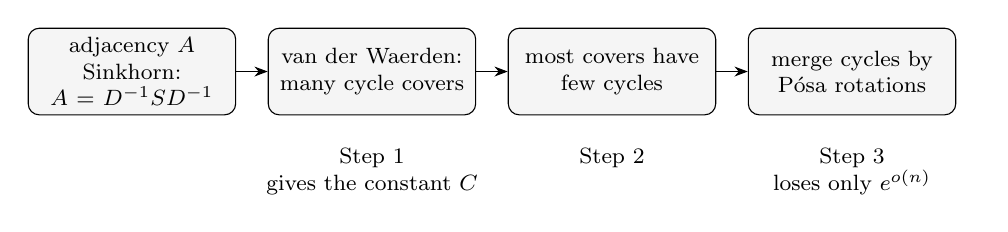
\begin{tikzpicture}[node distance=4mm and 4mm,
 box/.style={draw,rounded corners,align=center,fill=gray!8,minimum height=11mm,text width=24mm,font=\footnotesize},
 >={Stealth}]
\node[box] (a) {adjacency $A$\\Sinkhorn: $A=D^{-1}SD^{-1}$};
\node[box,right=of a] (b) {van der Waerden:\\many cycle covers};
\node[box,right=of b] (c) {most covers have\\few cycles};
\node[box,right=of c] (d) {merge cycles by\\Pósa rotations};
\draw[->] (a)--(b); \draw[->] (b)--(c); \draw[->] (c)--(d);
\node[below=3mm of b,font=\footnotesize,text width=30mm,align=center] {Step 1 \\ gives the constant $C$};
\node[below=3mm of c,font=\footnotesize] {Step 2};
\node[below=3mm of d,font=\footnotesize,text width=30mm,align=center] {Step 3 \\ loses only $e^{o(n)}$};
\end{tikzpicture}
\end{center}
\medskip
Cycle covers of the directed version of $G(n)$ are exactly the permutations $\pi$ with
$i\sim\pi(i)$ for all $i$. Their number is $\operatorname{per}(A)$.
\end{frame}

%=====================================================================
\begin{frame}{Step 1: permanents give exactly the constant $C$}
\textbf{van der Waerden} (Egorychev, Falikman 1981): if $S$ is doubly stochastic, then
$\operatorname{per}S\ge n!/n^n$.

\medskip
Scale $A=D^{-1}SD^{-1}$ with $S$ doubly stochastic, $D=\mathrm{diag}(d_i)$:
\[
\operatorname{per}A=\frac{\operatorname{per}S}{\prod_i d_i^2}\ \ge\ \frac{n!}{n^n}\prod_i d_i^{-2}.
\]
\textbf{If} the discrete scaling tracks the continuum one,
$d_i\approx n^{-1/4}a(i/n)$, then
\[
\log\operatorname{per}A\ \ge\ \log n!-\tfrac n2\log n+C\,n+o(n).
\]
\begin{block}{Lemma L1 (needed)}
The Sinkhorn scaling of $A_{G(n)}$ satisfies $\frac1n\sum_i\log\bigl(n^{1/4}d_i\bigr)\to\int_0^1\log a$.
This is an equidistribution statement for squares; the degrees carry no residue bias.
\end{block}
Together with Bregman: $\operatorname{per}A$ is then pinned between the constants $C$ and $B$.
\end{frame}

%=====================================================================
\begin{frame}{Steps 2 and 3: few cycles, then merge}
\begin{columns}
\column{0.5\textwidth}
\textbf{Step 2 (L2).} Under the $\kappa$-tilted measure, covers with more than $s=o(n/\log n)$
cycles carry a negligible fraction of $\operatorname{per}A$. (For a uniform permutation,
typically $\sim\log n$ cycles.)

\medskip
\textbf{Step 3 (L3).} Merge $s$ cycles into one Hamiltonian cycle by changing $O(s)$
edges. The map is at most $n^{O(s)}$-to-one, so the loss is $e^{O(s\log n)}=e^{o(n)}$.
\column{0.5\textwidth}
\textbf{Pósa rotation}
\begin{center}
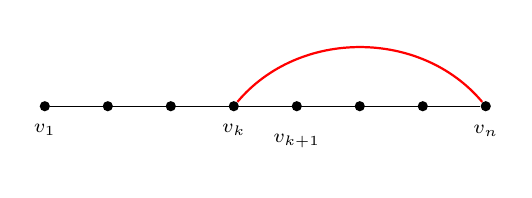
\begin{tikzpicture}[scale=0.8,every node/.style={circle,fill,inner sep=1.3pt}]
\foreach \i in {0,...,7} \node (p\i) at (\i,0) {};
\draw (p0)--(p7);
\draw[red,thick] (p7) to[bend right=50] (p3);
\node[draw=none,fill=none,below] at (p0.south) {\scriptsize $v_1$};
\node[draw=none,fill=none,below] at (p3.south) {\scriptsize $v_k$};
\node[draw=none,fill=none,below] at (p4.south) {\scriptsize $v_{k+1}$};
\node[draw=none,fill=none,below] at (p7.south) {\scriptsize $v_n$};
\end{tikzpicture}

\medskip
$\Downarrow$ \ delete $v_kv_{k+1}$, add $v_nv_k$

\medskip
{\small $v_1\cdots v_k\,v_n v_{n-1}\cdots v_{k+1}$: new endpoint $v_{k+1}$}
\end{center}
Repeated rotations give many endpoints; an endpoint adjacent to another cycle
lets you \emph{extend}.
\end{columns}
\end{frame}

%=====================================================================
\begin{frame}{Where the arithmetic bites}
Rotation--extension needs \textbf{expansion}: small sets have many neighbours, and
any two large sets are joined by an edge.

\medskip
$G(n)$ fails the second property:
\begin{itemize}
\item $\{i\equiv1 \bmod 3\}$ is an independent set of size $\approx n/3$;
\item there are no edges between $\{i\equiv0\}$ and $\{i\equiv2\} \pmod 4$.
\end{itemize}
\pause
But the \textbf{quotient graphs} on residue classes are connected:
\[
\bmod 4:\ 0\!-\!0,\ 0\!-\!1,\ 1\!-\!3,\ 3\!-\!2,\ 2\!-\!2,\qquad
\bmod 3:\ 0\!-\!0,\ 0\!-\!1,\ 1\!-\!2,\ 2\!-\!2 .
\]
\begin{block}{Lemma L3 (needed): residue-aware expansion}
Large sets that are ``compatible'' in every residue quotient are joined by many edges, and
rotations can be routed through allowed residue pairs.
\end{block}
This is the analytic number theory input (squares in residue classes and short
intervals), and it is where the real work lies.
\end{frame}

%=====================================================================
\begin{frame}{Summary}
\small
\begin{tabular}{@{}ll@{}}
\toprule
$\Ham(N)\ge 2^{(4N+2)/91}$, $N=(91\cdot25^m-1)/2$ & \proved\ \computed\\
$\log\Ham(n)\le\frac n2\log n+(B-1)n+o(n)$, $B=-0.61495$ & \proved\\
$\sqrt n\,G(n)\not\to\kappa$ \proved; limit on $[0,1]\times\Zhat$ & \conj\\
$\log\Ham(n)=\log n!-\frac n2\log n+Cn+o(n)$, $C=-0.63254$ & \conj\ fits $n\le74$\\
L1 $+$ L2 $+$ L3 $\Rightarrow$ lower bound with constant $C$ & \heur\\
\bottomrule
\end{tabular}

\medskip
\textbf{Open:}
\begin{itemize}
\item Exponential lower bound for \emph{all} large $N$ (Gerbicz's general step).
\item Prove L1, L2, L3; even $\log\Ham(n)\ge(\frac12-\varepsilon)n\log n$ would be new.
\item Does the arithmetic affect the constant? (Prediction: no.)
\item Recompute $\Ham(75)$.
\end{itemize}
\end{frame}

%=====================================================================
\begin{frame}[allowframebreaks]{References}
\footnotesize
\begin{itemize}
\item Á. Backhausz, B. Szegedy, Action convergence of operators and graphs, \emph{Canad. J. Math.} 74 (2022).
\item C. Borgs, J. Chayes, H. Cohn, Y. Zhao, An $L^p$ theory of sparse graph convergence I, \emph{Trans. AMS} 372 (2019).
\item L. M. Bregman, Some properties of nonnegative matrices and their permanents, \emph{Soviet Math. Dokl.} 14 (1973).
\item B. Cuckler, J. Kahn, Hamiltonian cycles in Dirac graphs, \emph{Combinatorica} 29 (2009).
\item G. P. Egorychev (1981); D. I. Falikman (1981): van der Waerden's conjecture.
\item R. Gerbicz, The square-sum problem, mersenneforum.org (2018).
\item R. Glebov, M. Krivelevich, On the number of Hamilton cycles in sparse random graphs, \emph{SIAM J. Discrete Math.} 27 (2013).
\item R. Kenyon, D. Král', C. Radin, P. Winkler, Permutations with fixed pattern densities, \emph{Random Struct. Alg.} 56 (2020).
\item M. Krivelevich, On the number of Hamilton cycles in pseudo-random graphs, \emph{Electron. J. Combin.} 19 (2012).
\item D. Kunszenti-Kovács, L. Lovász, B. Szegedy, Measures on the square as sparse graph limits, \emph{JCTB} 138 (2019).
\item L. Lovász, \emph{Large Networks and Graph Limits}, AMS (2012).
\item L. Pósa, Hamiltonian circuits in random graphs, \emph{Discrete Math.} 14 (1976).
\item R. Sinkhorn, \emph{Ann. Math. Statist.} 35 (1964); C. Léonard, the Schrödinger problem, \emph{DCDS-A} 34 (2014).
\end{itemize}
\end{frame}

\end{document}
